\section{Eye rendering}
One of the pitfalls of the model concerns the eye region: for different viewing angles, the eyes stay focused on the camera. In the 3D head models, it can be seen that the eye sockets are concave, shown in figure \ref{fig:concave_eyes}.

\begin{figure}[H]
\centering
  \centering
  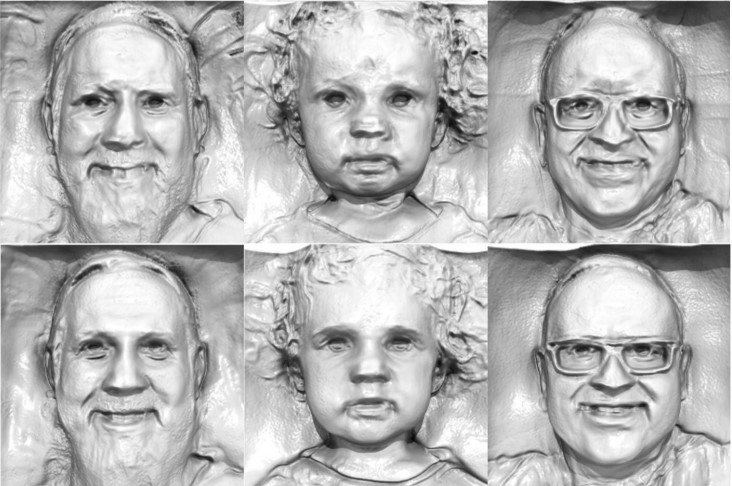
\includegraphics[width=.9\linewidth]{concave_eyes.jpg}
  \caption{3D rendered eyes showing the concave eye area \cite{chan2022efficient}}
  \label{fig:concave_eyes}
\end{figure}

When creating the 2D images from different viewing angles, the model interprets this incorrectly, locking the eyes to the camera in every pose. A reason can not be found in literature. However, we believe the reason for this is the training data. In mostly all training images, the person looks towards the camera. Therefore the model makes all the output images look at the camera as well. This could be tested by training the model on a more uniformly distributed set of people looking towards the camera and people looking away from the camera. \\
However, a definite answer to the lower density in the eye part has not been found yet. To try to solve this problem, the first step is to prepare a dataset on this specific area. As the model is trained on the full head, it is not possible to change the model's output to only the eyes without retraining the model. Instead, the eye portion is extracted from the full 3D head and only that part is rendered with the computer graphics algorithm Marching cubes (figure \ref{fig:eye_rendering_step}). The resulting 3D model can be seen in figure \ref{fig:cropped_eyes}.

\begin{figure}[H]
\centering
  \centering
  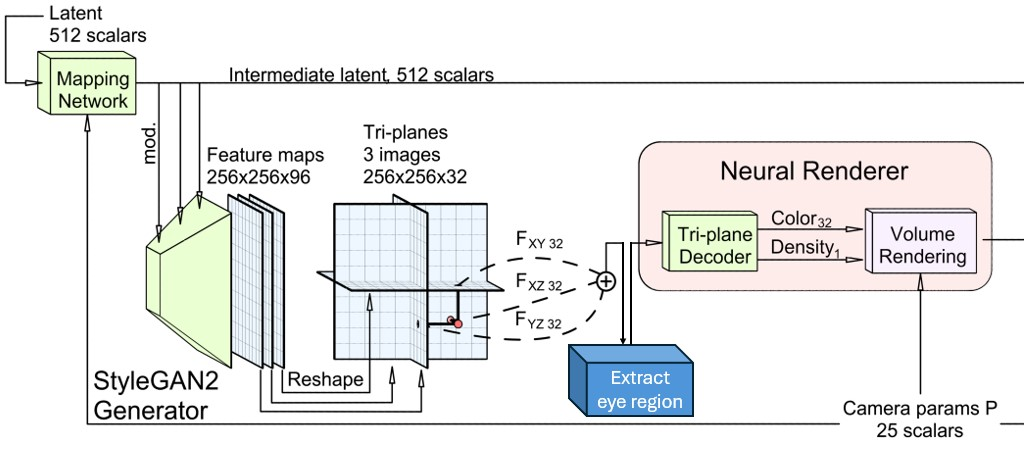
\includegraphics[width=.6\linewidth]{eye_rendering_step.jpg}
  \caption{Framework with the additional step to extract the eye region}
  \label{fig:eye_rendering_step}
\end{figure}

\begin{figure}[H]
\centering
  \centering
  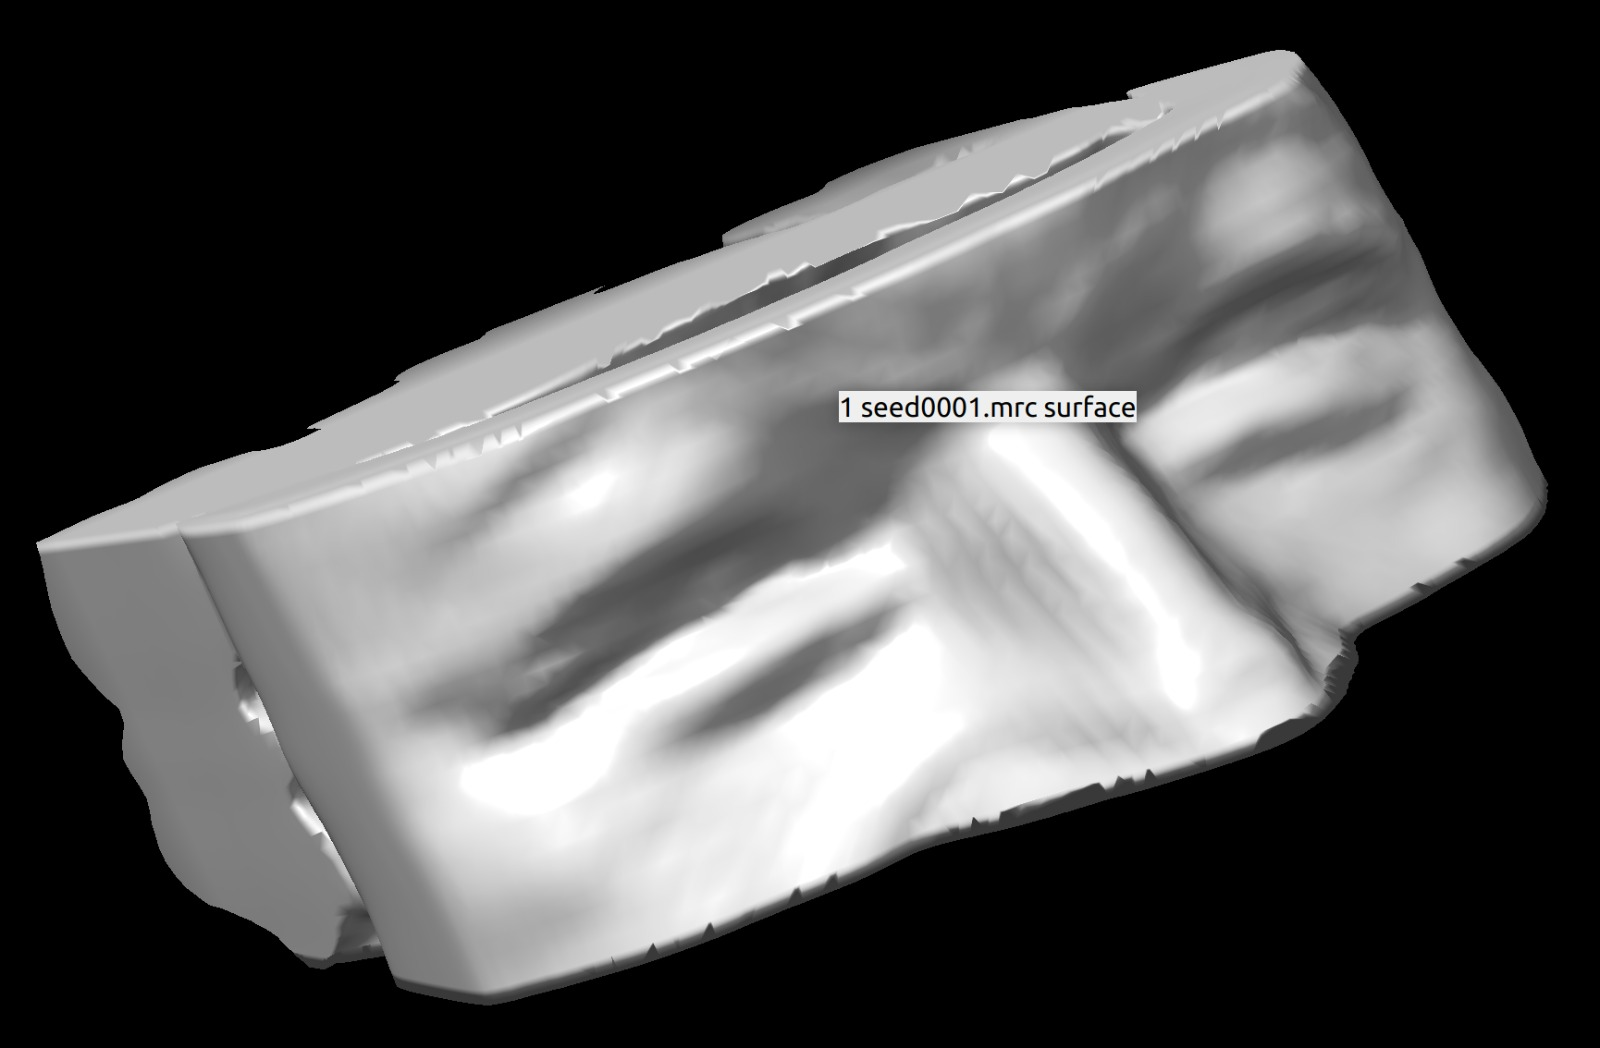
\includegraphics[width=0.7\linewidth]{Cropped eyes.jpg}
  \caption{Cropped 3D model of only the eyes}
  \label{fig:cropped_eyes}
\end{figure}

\subsection{3D Eye model}
Now that we know how to use the extracted 3D eye region, we need to find a way to obtain these 3D models. When the full head is modeled, it starts building in the bottom left corner, and adds 'blocks' in vertical strokes. To build only the eye region, we adapted the code to start at the top of the left cheek and work its way up to above the eye. By exhaustive exploration we have found that the bottom 50\% of the face is redundant. The same goes for the top 37\%. These values leave some space above and below the eyes, which is what makes them generalizable. For all faces that we have tested, the eyes fall within this region without leaving large margins on either side of the eye. For the specific changes in the code, please read the commit changes of our solution \parencite{gitcommit}.